\section{Design}
In order to measure the enjoyability of a location-based game (LBG) with a game activity as the navigational method between POIs, we developed a LBG. The game takes place in Aalborg, Denmark and the points of interest (POIs) are three street art paintings\cite{streetart}. The game makes players walk between the three POIs on a route with a total length of 1.8km and a distance of 0.9km between POIs (see Figure \ref{FinalRoute}). Due to requirements from the method of the experiment as described in (INSERT REFERENCE TO METHOD SECTION), the particular route was chosen on the basis of it having approximately the same amount of intersections in the road between POIs as well as approximately the same distance between the POIs.

\begin{figure}[hbtp]
\centering
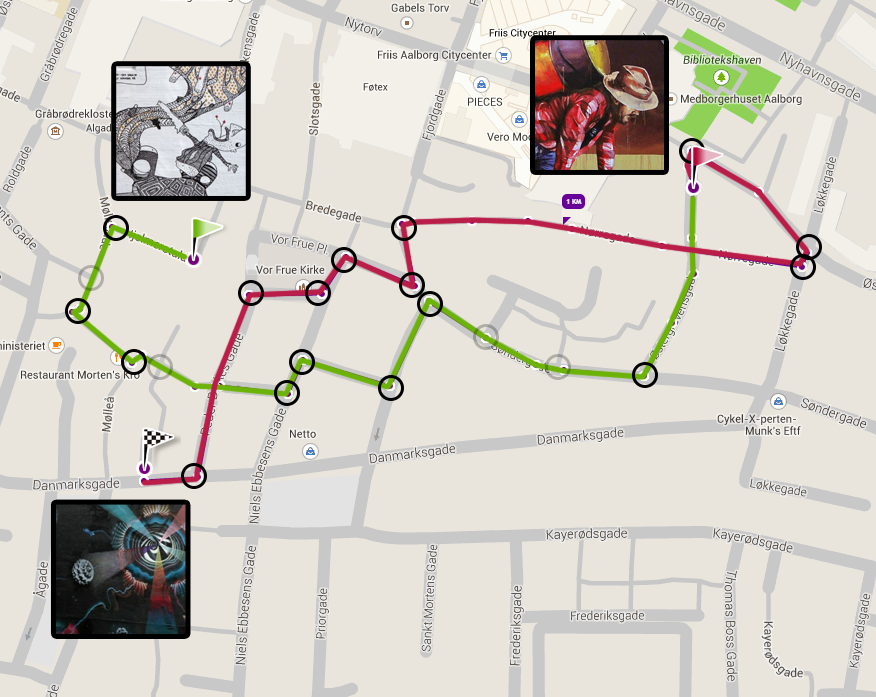
\includegraphics[scale=0.2]{Pics/FinalRoute.png}
\caption{The route between the three street art paintings.}
\label{FinalRoute}
\end{figure}

\subsection{Choice of Navigational Game Activity}
In the process of designing the navigational game activity using landmarks, four initial designs were created as paper prototypes and one was chosen to be used in the game on the basis of three initial tests of the designs. The tests were done using within-subjects design, meaning that each group of participants used a specific navigational game activity for each quarter of the route. The purpose of the tests was to determine which game activity the participants found most enjoyable, based on short semi-interviews conducted between game activities as well as after trying all four activities. The participants of each test were a child in the age group of 8-11 years and the child's parent. We followed the participants during the activities, documenting the tests and interfering if they got lost or had other problems. As the initial designs were paper prototypes with a focus on the navigation, it must be noted that elements of LBGs such as a feedback system, a narrative, activity at POIs, and learning were not a part of the experience in these initial tests.

When designing the four navigational game activities, inspiration was taken from popular children's games, since they are familiar to most children, causing a lower learning curve for the families. Similar game activities were also found in other LBGs, giving inspiration for how they should be used in a LBG. Three navigational game activities were made as variations of matching card games such as \textit{Concentration}\cite{childrensGames}. In these types of games, players specify two or more cards that are alike, among a set of cards, and the goal is typically to be the player with the most matches in the end. In Team Exploration\cite{GamingOnTheMove}, players match pictures in the virtual space to landmarks in the physical space and progress in the game by specifying which pictures belong to certain areas of a map. Similarly, players are given pictures of landmarks in our three matching game activities; \textit{Simple Matching}, \textit{Order Matching}, and \textit{Memory Matching}.

For all four game activities, local landmarks are used to help players choose directions at decision points, and route marks are used along streets to confirm to players that they are walking in the correct direction. In Simple Matching, players are given a set of potential landmarks, where only one of them is a true landmark in their current location. When they spot or match the landmark that is shown on the picture, they go to its position and start matching the next set of pictures. This activity proved to be the easiest of the four and most participants found it to be uninteresting due to its lack of challenge. Order Matching is very similar to Simple Matching, as the only difference is that players have to specify the order in which the presented landmarks occur from their current position. Participants found this activity to be a bit more challenging, however due to the requirement of ordering landmarks, participants sometimes walked back in the direction they came from. Through observation, it was clear that the participants collaborated more in this activity due to the increase in difficulty. In Memory Matching, the landmarks to be ordered are only presented quickly before navigating. When participants then reach the last picture in the set, they are asked to specify the order of landmarks encountered. Through observation and interviews, it was clear that participants found this activity to be the most challenging of all matching activities. This also caused participants to collaborate more, where they e.g. each would remember half of the pictures. Furthermore, participants mentioned that only being able to look at the pictures at certain points, caused them to look more around and notice the environment during navigation.

The last game activity designed was based on riddles, where similar to the game \textit{I Spy}\cite{childrensGames}, players must spot a specific object in the vicinity based on a sentence hinting about attributes of the object. Based on I Spy and the LBG CityTreasure, where riddles are used at POIs, we designed an activity where riddles hint about the next landmark to go to. As in I Spy, the riddles describe attributes of objects through hints.

In the context of landmarks, the riddles describe saliency based on the visual, cognitive or structural attributes of the landmark, either in isolation or in combination. In order for players to confirm that they have found the landmark, they are also given a control question about the landmark with three possible answers. This was a solution to the problem of specifying the players' exact position through GPS, since at the time of designing the activity, it had been observed that accurate positions could not be given through GPS. Furthermore, this control question allows for the possibility of including knowledge about the landmarks in the game activity, thereby supporting pedagogic elements in the game. By being able to confirm if the player has found the landmark, it is possible to create a feedback system in the game. Upon answering the control questions, regardless of the players' answer, a picture of the correct landmark is shown to the players, so they never get lost. Through interviews, it was found that most participants preferred navigation with riddles due to them being the most fun. It was also clear that of all activities, riddles were the most challenging for the participants, mainly because people were unsure of the scale in which the landmarks could be found. This is due to the fact that participants have nothing visual to compare to in opposition to the matching activities. However, it could also be seen that this limitation contributed to the enjoyability of the activity. We also observed that this limitation caused participants to collaborate and in general communicate more during navigation. Based on these results, there were strong indications that navigation using riddles was the most enjoyable activity. For this reason, riddles were chosen as the navigational game activity to be used in our experiment. In order to test the navigational game activity in the context of LBGs, a LBG was developed.

\subsection{Lost on Earth}
\textit{Lost on Earth} builds on the LBG \textit{Monsters Eat Art}\cite{Lynge}
Built on Monsters Eat Art -> target group
Have to help the monster
Narrative including street arts
